%% This is an example first chapter.  You should put chapter/appendix that you
%% write into a separate file, and add a line \include{yourfilename} to
%% main.tex, where `yourfilename.tex' is the name of the chapter/appendix file.
%% You can process specific files by typing their names in at the 
%% \files=
%% prompt when you run the file main.tex through LaTeX.
%% prompt when you run the file main.tex through LaTeX.
\chapter{Predicting Mercury Concentrations in the Atmosphere in Latin America using GEOS-Chem }
%% BACKGROUND
\section{Background}
\begin{flushleft}

Chemical transport models such as GEOS-Chem provide an approximation of the behavior of various chemical species in the atmosphere that enables understanding of the real world and creates opportunities for future predictions. Moreover, model outputs being approximations means that they are inherently error prone and these errors must be identified, quantified and minimized to improve the model's usefulness. In order to evaluate the model errors and identify unexpected behaviors, comparison of the model outputs with observations of the atmosphere is critical \cite{brasseur_modeling_2017}. Therefore, models and observation networks have a symbiotic relationship that is one of the cornerstone ingredients of the multidisciplinary frameworks for producing scientific information and knowledge that is salient, credible and legitimate to inform the public and policy makers. According to Cash et al.,(2003), science is likely to influence social responses to public issues when relevant stakeholders consider it credible, salient, and legitimate\cite{cash_salience_2003}. Comparisons of model output with observations address the credibility aspect, which is concerned with the scientific adequacy of the technical evidence \cite{cash_salience_2003}.Furthermore, Cash et al., (2003) argue that systems that actively and consciously manage the multiple boundaries within the system and balance trade-offs between salience, credibility, and legitimacy are more effective than those that do not \cite{cash_salience_2003}. Considering Cash et al., (2003)'s proposition together with Brasseur et al. (2017)'s description of models as a common platform for the integration of information from instruments measuring different species and operating  on platforms with different measurement locations and schedules, model observation comparison is an important form of effective boundary management. 
\end{flushleft}

\begin{flushleft}
An ensemble of observations helps check consistency of observations and enables constraints from multiple sources to be considered in evaluating the model\cite{brasseur_modeling_2017}.Therefore, numerous studies comparing different Hg model outputs to Hg observation have been published which has improved our understanding of the biogeochemical cycle of Hg. As an example, Chapter 5 of the GMA 2018 analyzes model and measurement studies that address many aspects of Hg transport and fate. These include emissions, atmospheric chemistry, removal processes, modeling, and historical trends. Moreover, region specific modelling studies are presented featuring the polar regions, Europe, North America and East Asia. However, no detailed modelling studies are presented for some of the regions that are reported to have high anthropogenic Hg emissions as seen on Figure \ref{fig:world_hg_emisions}. We also scanned numerous modelling studies to identify the extent to which regions such as Latin America, Africa and South East Asia are analyzed in the context of model observation comparison and the analysis in this thesis is one on the few literature sources that deliberately target one of those regions, Latin America. 
\end{flushleft}

\begin{figure}[H]
  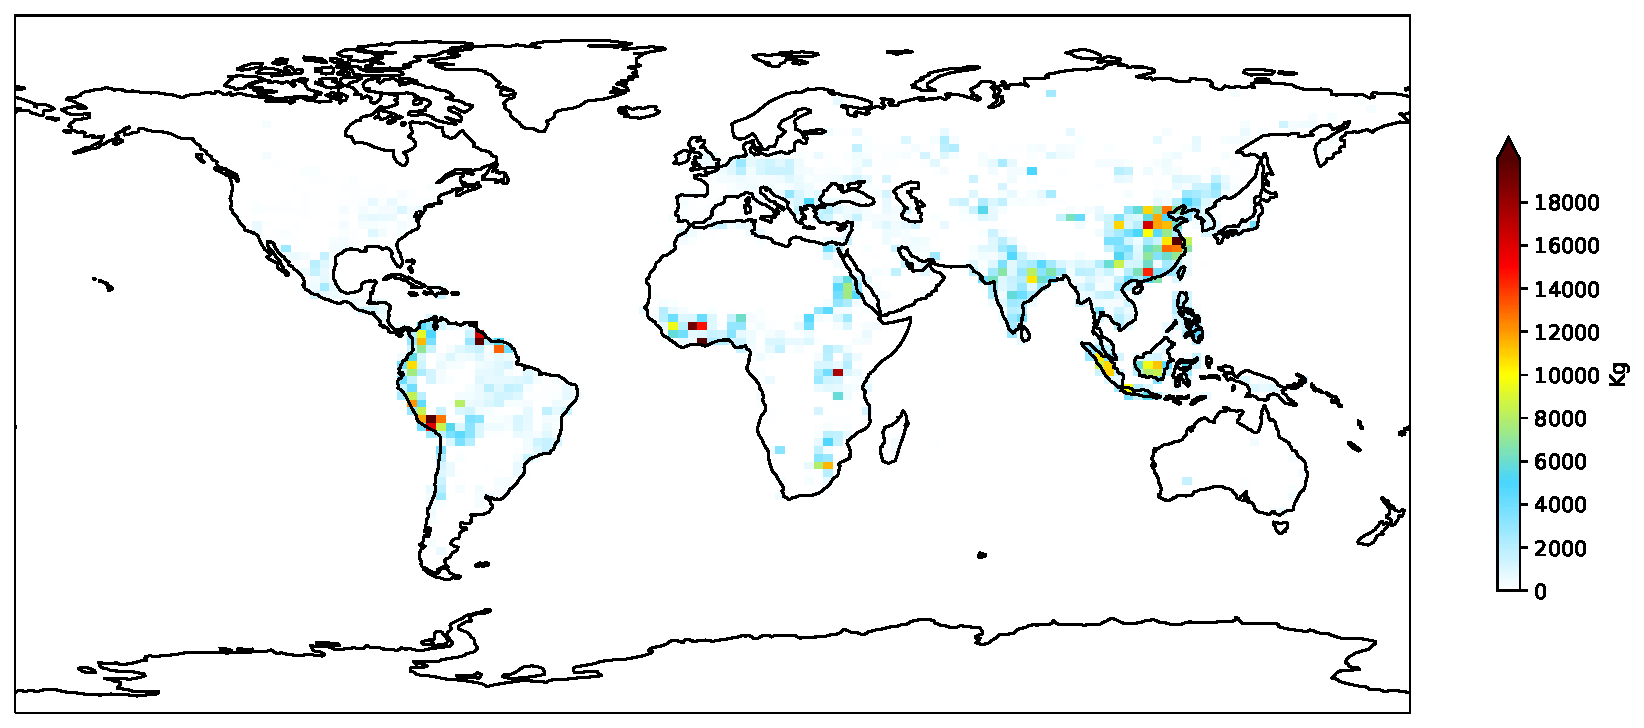
\includegraphics[width=0.8\textwidth]{templates/figures/06-12-22_total_Hg0-emissions-per-year_globally_001.pdf}
  \centering
  \caption{Spatial distribution of annual average Hg anthropogenic emissions for a year period between July 2014 and July 2015}
  \label{fig:world_hg_emisions}
\end{figure}
\FloatBarrier


\begin{flushleft}
Additionally, the Madre de Dios region was estimated to have released the largest quantities of Hg to the environment and the atmosphere. Madre de Dios whihc is shown by the red outline in Figure \ref{fig:PeruCS} is a rain forest region that lies between Bolivia and Brazil and covers roughly 85,000 square kilometers . The region's name is derived from the name of a major river that runs through it, and smaller streams and rivers cross through it to provide transportation and fishing for indigenous communities. Furthermore, these waterways are the main sites of ASGM and, subsequently, Hg contamination. Hg has been extensively studied in Madre de Dios, both in people and in the environment \cite{ashe_elevated_2012}\cite{moody_mercury_2020-1}.

\end{flushleft}

\begin{flushleft}
\begin{figure}[H]
  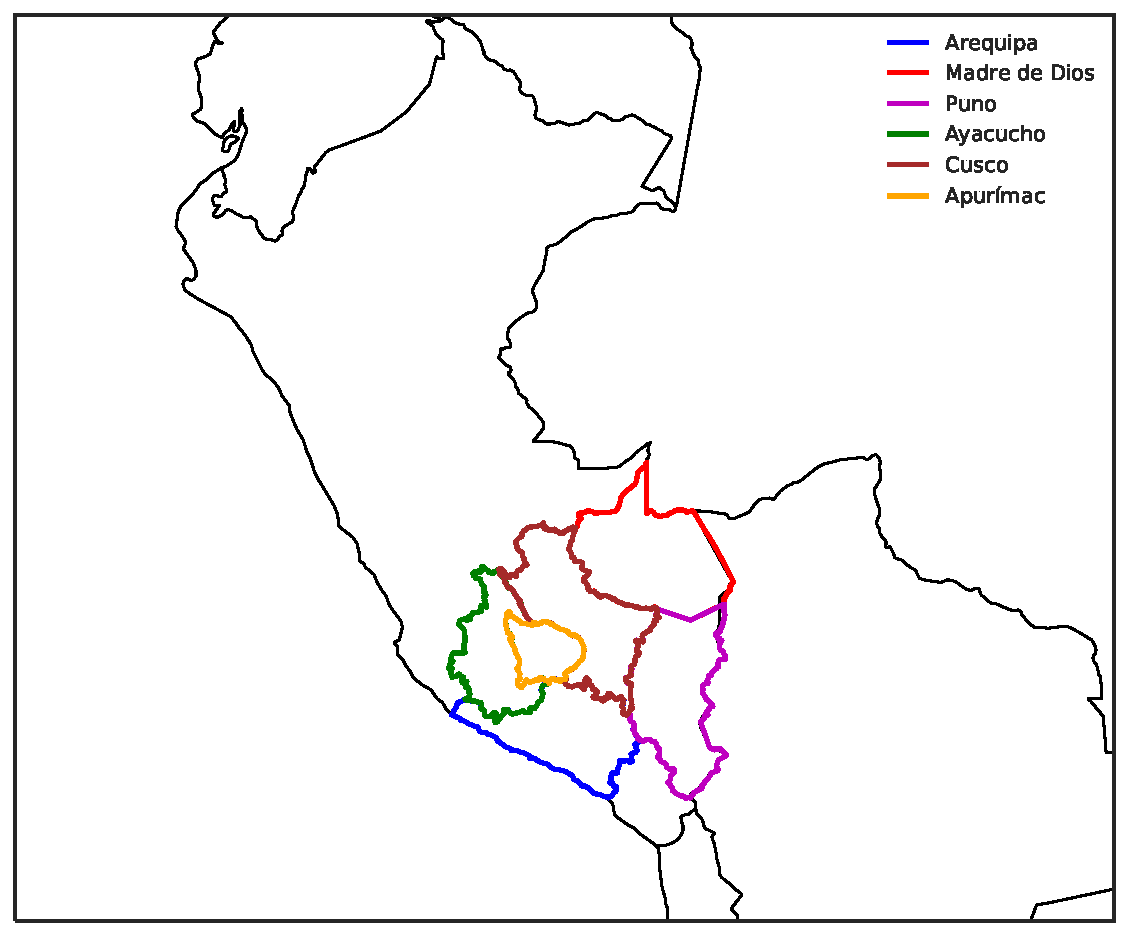
\includegraphics[width=0.6\textwidth]{templates/figures/Peru_Maps/CasestudyRegion.pdf}
  \centering
  \caption{Departments predicted to be the prominent sources of ASGM Hg releases according to the Artisanal Gold Council's  Inventory Report for the ASGM sector in Peru (2017) }
  \label{fig:PeruCS}
\end{figure}
\FloatBarrier

Prior environmental measurements performed in Madre de Dios regarding the amount of Hg entering soil, air, and waterways reflected drastically different results between government estimates and international researchers. This demonstrates a need to generate further system-wide constraints on ASGM Hg use and pollution. This thesis project complements previous studies and distinguishes itself from previous studies in this highly-studied region by investigating the extent to which the GEOS-Chem model can leverage existing measurements of Hg int the atmosphere and Hg emission estimates in published Hg global and national inventories to develop constraints on the amount of ASGM Hg emission in Peru. To develop a comprehensive understanding of how Hg pollution impacts the environment, long-term monitoring of ambient Hg data on a global scale is vital to assessing its emission, transportation, atmospheric chemistry, and deposition processes. Brasseur et al., (2017) assert that having a large ensemble of observations is vital for model evaluation; hence the lack of studies that analyze Latin America, Africa and South East Asia may be attributed to the fact that the aforementioned regions historically did not have enough Hg monitoring capacity. Although, a notable number of new atmospheric Hg monitoring programs have been set up and monitoring data from Latin America published in the last few years, Latin America, Africa and South East Asia are significantly behind Europe, and North America regarding capturing the relevant observation ensembles. Regardless of the dearth of a large ensemble  of observations in Latin America, we present analysis and evaluation of Hg  concentration measurements recorded at multiple sites in Latin America including gaseous elemental mercury (GEM) concentration data form a network of passive air samplers (PAS). 
\end{flushleft}



%%----------------------------METHODS-------------------------------------------
\section{Methods}
\subsection{GEOS-Chem}
\begin{flushleft}
The GEOS-Chem model (Bey et al., 2001) is used to simulate atmospheric concentrations of Hg for comparison with data constraints. GEOS-Chem is a global-scale, 3-D atmospheric chemical transport model driven by meteorological input from the Goddard Earth Observing System (GEOS) of the NASA Global Modeling and Assimilation Office. It runs at a resolution of 0.25° latitude x 0.3125° longitude horizontally, equivalent to $\approx$27 km at the equator, and 72 levels in the vertical. Numerous atmospheric chemical species have been simulated using GEOS-Chem, including Hg (Selin et al., 2008, Zhang et al., 2016, Selin et al., 2007, Holmes et al., 2010, Amos et al., 2012). Travnikov et al. (2017) also used GEOS-Chem for international model comparisons to support the Global Mercury Assessment and the Minamata Convention on Mercury.
Herein we simulated the Hg concentration in the atmosphere using version 12.8.0 of GEOS-Chem at a resolution of 2.0$\times$2.5, which is equivalent to a 200 km$\times$250 km grid square at the equator. Furthermore, the GMA 2018 emissions inventory was used to represent anthropogenic emissions sources from all sectors. Different inputs to the GEOS-Chem model such as emissions sources can be toggled on or off depending on the research objective, hence a baseline simulation was created by turning on all Hg emissions sources globally. Moreover, a \off was generated by turning off the ASGM source globally to evaluate the contribution of ASGM to the baseline \hg in the atmosphere by calculating difference between the \on and \off.
\end{flushleft}

\begin{table}[H]
\captionof{table}{Description of GEOS-Chem Simulations Conducted}
\label{tab:geos_chem_simulation_description}

\centering
\resizebox{\textwidth}{!}{\begin{tabular}{lcp{0.6\linewidth}}

Simulation Name  & Resolution & Description  \\
                        
\hline
Base (ASGM=ON)         & 2.0$\times$2.5 & All Hg anthropogenic emission sources are turned on  \\
Base (ASGM=OFF)        & 2.0$\times$2.5 & All Hg anthropogenic emission sources are turned on except ASGM emissions 

\end{tabular}}

\end{table}

\begin{flushleft}

 The frequency of the simulation output set set to output daily \hg averages at the global scale while the \hg output for the grid boxes corresponding to the locations of the observation sites was set to a hourly frequency. The GEOS-Chem outputs for all the simulations conducted were in units of parts per trillion (ppt) and were converted to \ng to compare them to observations.
\end{flushleft}

\subsection{Observation Data}
\begin{flushleft}
As reported in the GMA 2018 and depicted on Figure \ref{fig:Latam_Hg_em}, Peru is one of the top emitters of ASGM related Hg \cite{united_nations_environment_programme_technical_2019} to the atmosphere. Yoshimura et al. (2021) estimated the mercury losses and gold production by ASGM and found that Latin America has the highest average ratior of Hg lost to gold produced as 4.63 in comparison to 1.96 in Africa and 1.23 in Asia. In South America, especially in tropical regions, atmospheric Hg data are rare; hence its dynamics are not well understood. 
\end{flushleft}
\begin{figure}[H]
  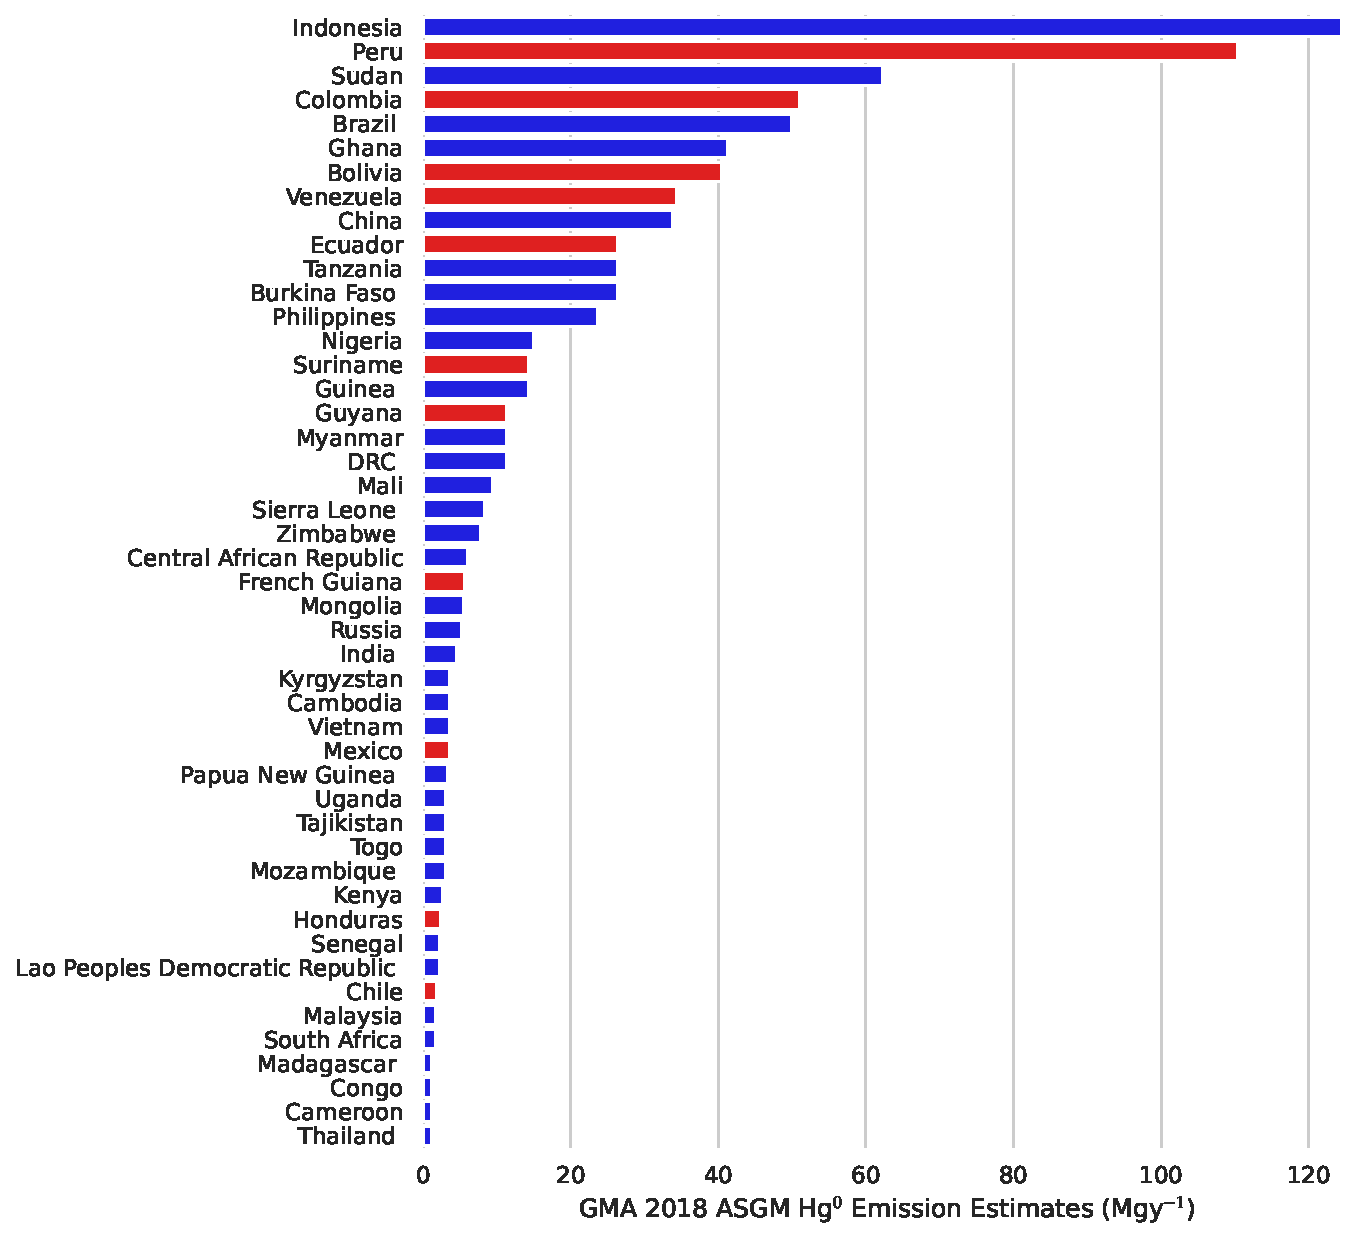
\includegraphics[width=\textwidth]{templates/figures/07-14-22_gma2018_top-asgm-emmiting-countries.pdf}
  \centering
  \caption{Bar chart showing the GMA 2018 ASGM \hg emission estimates for all countries in the world that have estimated ASGM \hg emissions above 1 Mg. The red bars indicate countries in Latin or South America }
  \label{fig:Latam_Hg_em}
\end{figure}
\FloatBarrier



\begin{flushleft}
 The Global Mercury Observation System (GMOS) is one of a few major global projects aimed at developing a global observing system for mercury pollution. A vast network of ground-based monitoring stations, regular oceanographic cruises, and lower, upper, and stratospheric measurements make up this European-funded project \cite{sprovieri_atmospheric_2016} \cite{koenig_seasonal_2021}. More than 40 ground-based monitoring sites constitute the international network, covering many regions with limited to no observational data available before GMOS. The GMOS monitoring network sites in Latin America are shown by the dots with red outline on Figure \ref{fig:GMOS_PAS_stations_map}. Available Hg observation data from the GMOS stations on Figure  \ref{fig:GMOS_PAS_stations_map} was obtained from the GMOS online database as well as published studies about the Hg monitoring data from the different sites. different sites\cite{koenig_seasonal_2021}. The hourly measurements of total gaseous mercury (TGM) in the atmosphere published in ngm\textsuperscript{-3} was retrieved from the GMOS online database, converted ti daily averages and compared to the GEOS-Chem modelled \hg at the various sites for the period between 2012 and 2016. 
\end{flushleft}

\begin{flushleft}
GEM monitoring equipment such as those used in the GMOS network can be prohibitively expensive, energy-intensive, and require extensive training. However, passive air samplers (PAS) require no energy to operate and do not require any special handling skills in addition to being a tool that can be easily deployed for long periods. This combination of attributes of PAS allows more sampling sites to be studied over a more extended period enabling significant average GEM concentration estimates to be obtained. Average annual GEM concentration data for 27 sites in Latin America as shown by the blue dots on Figure  \ref{fig:GMOS_PAS_stations_map} was obtained from the Wania Group at the University of Toronto. The PAS GEM data set included information about the coordinates of the deployment sites and the period of measurement. We compared the PAS data to the annual average concentration the year 2015 and the coordinate information from the PAS data was used for direct comparison of the GEM observations and model outputs at different sites.
\end{flushleft}

\begin{figure}[H]
  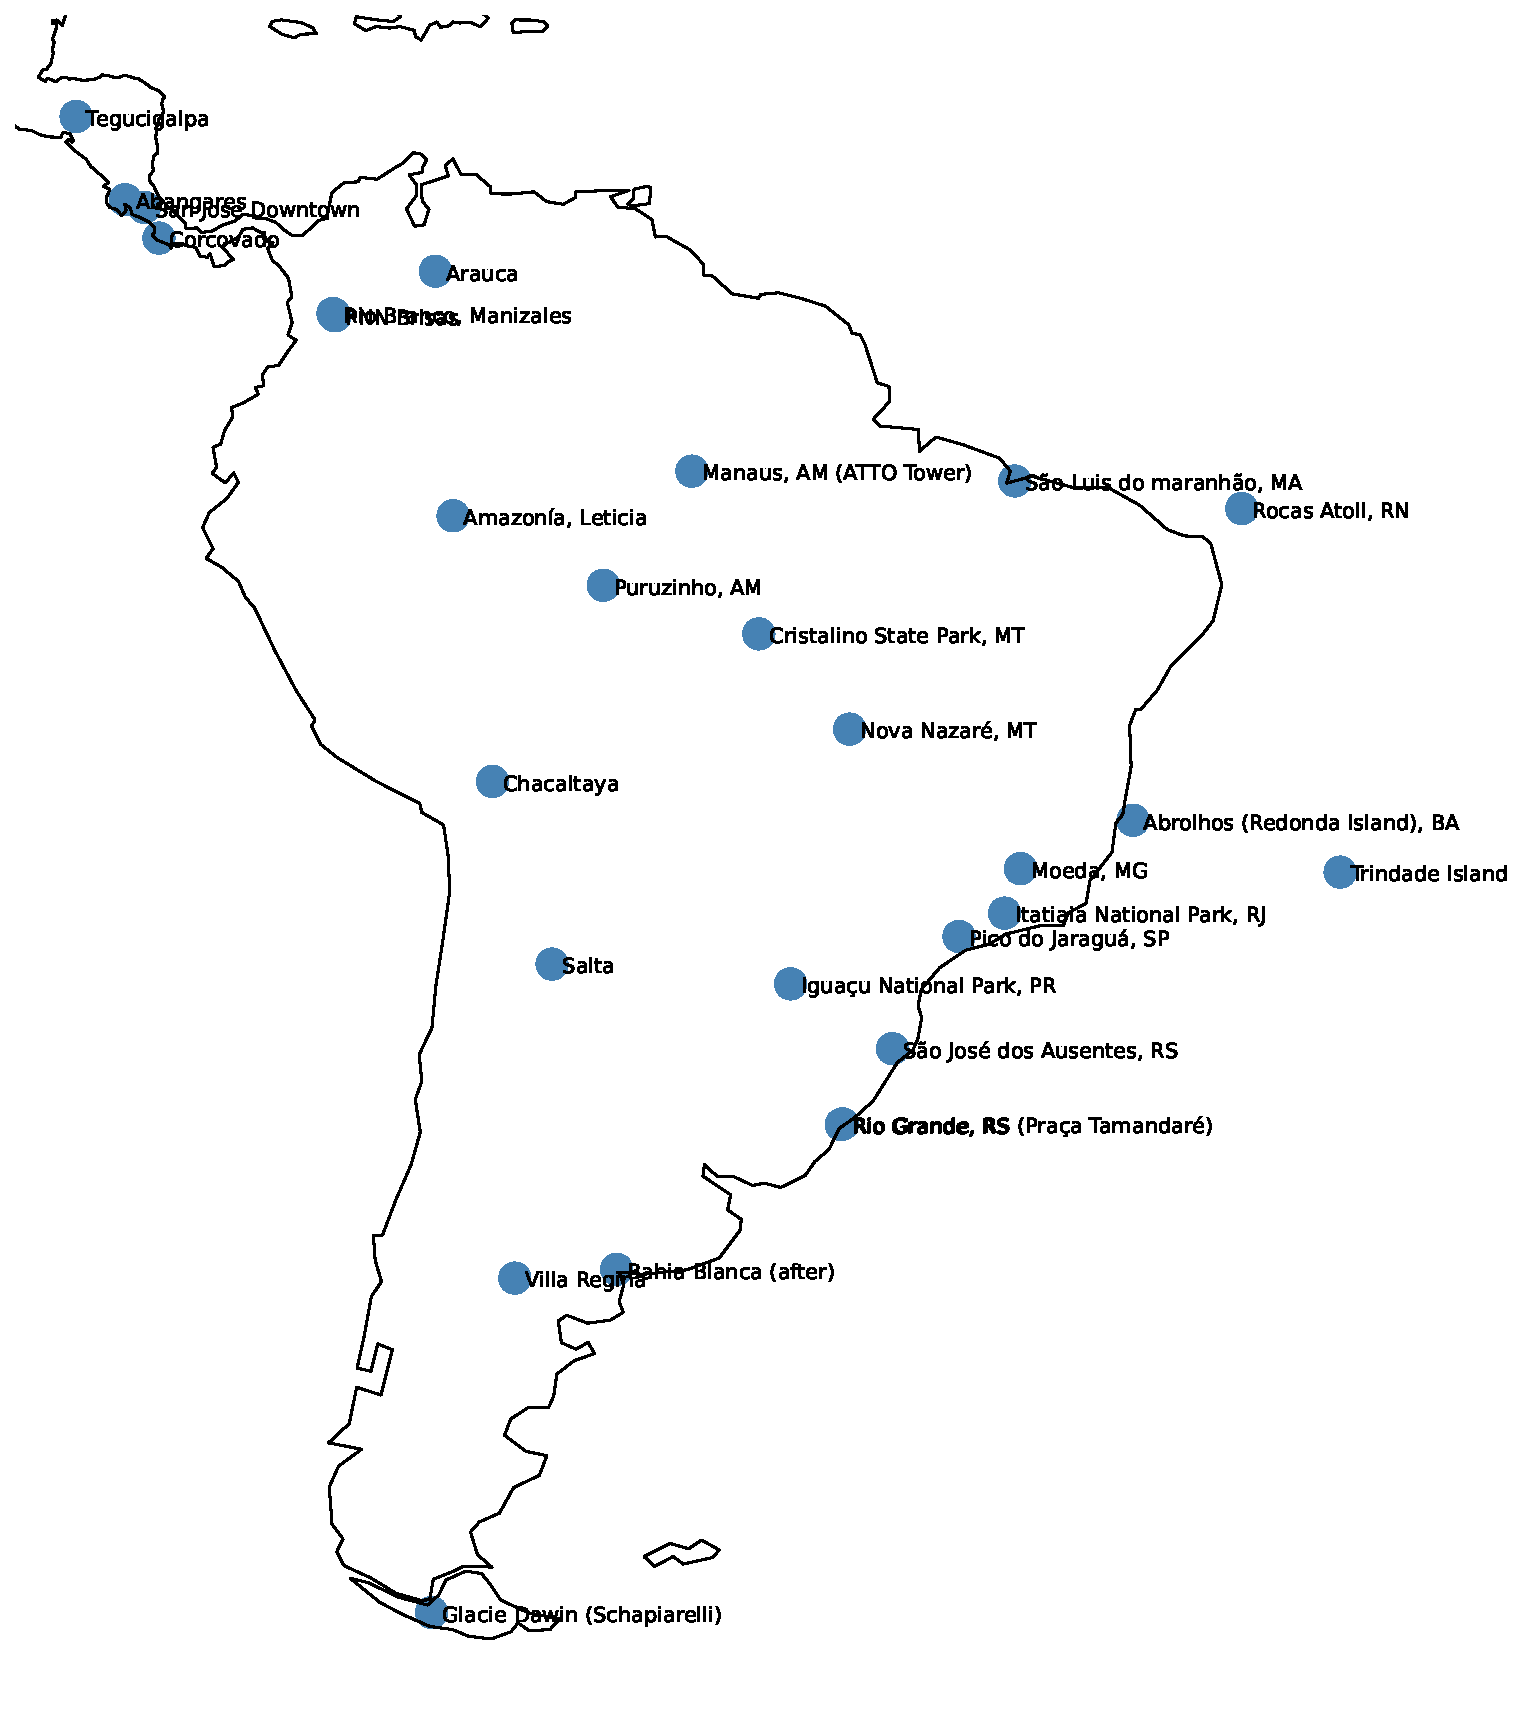
\includegraphics[width=0.8\textwidth]{templates/figures/Passive_Samplers/Latam_Passive_SamplerSites.pdf}
  \caption{Map Showing the GMOS Monitoring Network Sites and Passive Sampler Locations in South America}
  \label{fig:GMOS_PAS_stations_map}
  \centering
  
\end{figure}
\FloatBarrier







%%----------------------------RESULTS AND DISCUSSION---------------------------
\section{Results and Discussion}
\subsection{GMOS Observations vs GEOS-Chem}
\begin{flushleft}
Figure \ref{fig:GMOSvsGC} shows the average daily TGM concentration at the GMOS sites (red line) compared to the modeled \on average daily \hg shown(blue line) and the ASGM contribution (black line). The different Hg concentrations are plotted as a function of time based of the availability of data records between 2012 and 2016. None of the sites have a continuous data set that spans the entire measurement period but the Niew Nickerie and Manaus sites have the least data records at 215 and 100 respectively as seen on Table \ref{tab:ASGM_at_GMOS_annual_avs}. Moreover these two data sets have the worst mean and variability relationship with the modelled \hg as seen on Table \ref{tab:modelvsobs metrics}. Even though the GEOS-Chem model overestimates the mean concentration over a one year period of measurement with the exception of the Manaus site as seen in Table \ref{tab:ASGM_at_GMOS_annual_avs} the estimates for the mean concentration at Sisal and Calhau are within a 10\% margin as shown in Table \ref{tab:modelvsobs metrics}. However, the model grossly underestimates the variability in most of the GMOS sites except the Chalcataya site where the estimated standard deviation in within a 15\% margin.  
\end{flushleft}


\begin{figure}[H]
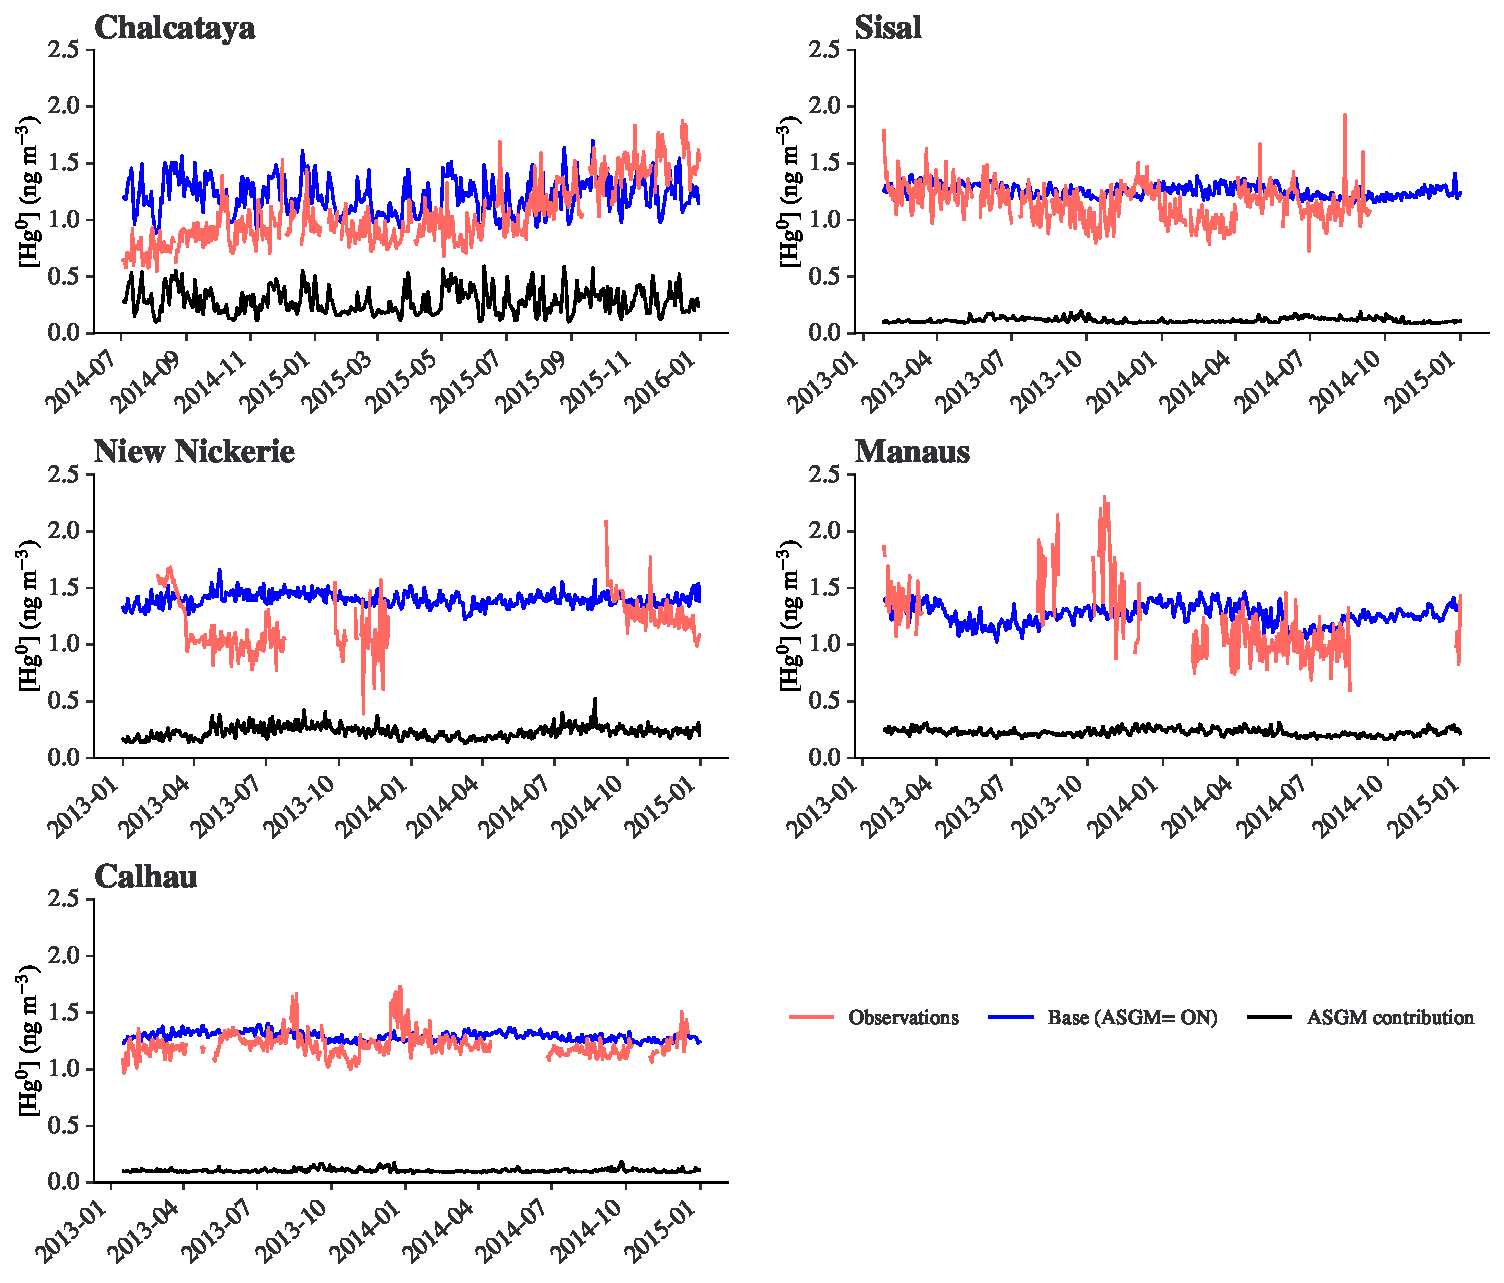
\includegraphics[width=\textwidth]{templates/figures/GMOS_Sites/GMOS_Sites.pdf}
\centering
\captionof{figure}{Plots time series plots of the observed TGM concentrations at different GMOS sites in red with the corresponding modeled concentration in blue and the associated ASGM contribution in black}
\label{fig:GMOSvsGC}
\end{figure}
\FloatBarrier

\begin{flushleft}
 Furthermore, the time series plot of the Hg concentrations at Chalcataya show a general upward trend that is not seen in the other observations and the also not predicted by the model. Table \ref{tab:ASGM_at_GMOS_annual_avs} compares the average  Hg concentration at the GMOS sites 
\end{flushleft}


\begin{table}[H]
\captionof{table}{The comparison of the model predictions of the average Hg concentration for a 1 year measurement period}
\label{tab:ASGM_at_GMOS_annual_avs}

\centering
\resizebox{\textwidth}{!}{\begin{tabular}{lcccccc}
  \hline

GMOS  &Number of& Observed Hg\textsuperscript{0} & Observation Standard & Base(ASGM=ON) Hg\textsuperscript{0} & Base(ASGM=ON) Standard  & ASGM Contribution  Hg\textsuperscript{0}   \\
Site & Records & (ng m$^{-3}$)/year             & Deviation ($\sigma$) & (ng m$^{-3}$)/year                   & Deviation ($\sigma$)      &(ng m$^{-3}$)/year\\
                        
\hline
Sisal          & 320 &1.19 & 0.14 & 1.27 & 0.05 & 0.12  \\
Calhau         & 309 &1.22 & 0.12 & 1.30 & 0.04 & 0.11  \\
Niew Nickerie  & 215 &1.11 & 0.23 & 1.41 & 0.06 & 0.25    \\
Manaus        & 100 &1.49  & 0.31 & 1.27 & 0.09 & 0.23   \\
Chalcataya     &333 &0.90 & 0.16 & 1.20 & 0.14   &0.28   \\
  \hline
\end{tabular}}

\end{table}
\begin{flushleft}
   The comparison of the GMOS observations to the GEOS-Chem model output, as seen in Figure \ref{fig:GMOSvsGC} indicated that the model generally over-estimates the observed Hg concentrations at the different GMOS sites.  With the exception of predicted concentration at the Chalcataya site, the modelled concentrations have low variability.  
\end{flushleft}

\begin{table}[H]
\captionof{table}{Table showing the extent to which the model predicts the observations showed by the percentage difference between the model predictions and the observations }
\label{tab:modelvsobs metrics}

\centering
\resizebox{0.5\textwidth}{!}{\begin{tabular}{lcc}
  \hline

GMOS  &Percentage difference & Percentage difference  \\
Site & annual mean (\%) & standard deviation (\%)           \\
                        
\hline
Sisal          & 6.72 &-64.29  \\
Calhau         & 6.56 &-66.66   \\
Niew Nickerie  & 27.03 &-73.91    \\
Manaus        & -14.77 &-70.97    \\
Chalcataya     &33.33 &-12.5   \\
  \hline
\end{tabular}}

\end{table}
\begin{flushleft}
 The extent of the  the ASGM emissions related Hg concentration signal created by the GEOS-Chem model is prominent in only one of the GMOS sites during the measurement periods we compared to the GEOS-Chem simulation. The site that had a prominent ASGM  is mountain site at the Chalcataya (CHC) regional station, Figure \ref{fig:GMOSvsGC} (a), (World Meteorological Organization, WMO, region III-- South America; 16.35023◦ S, 68.13143◦ W),which is at an altitude of 5240 meters above sea level, about 140m below the summit of mount Chacaltaya on the eastern edge of the ``Cordillera Real,'' with a horizon open to the south and west. CHC is about 300km from the ``Madre de Dios'' watershed.
\end{flushleft}

% \begin{figure}[H]

% \begin{tabular}[H]{cc}
% \setlength{\tabcolsep}{2.5pt}

% \subfloat[Chalcataya]{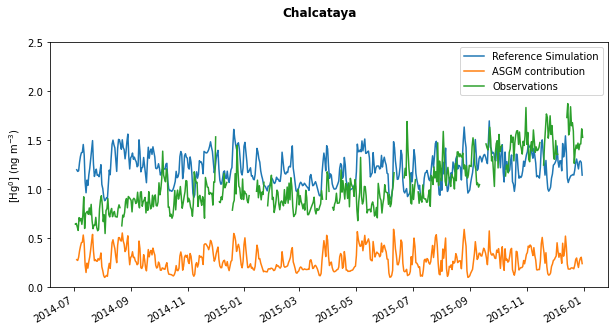
\includegraphics[width = 0.3\linewidth]{templates/figures/GMOS_Sites/chc.png}} &
% \subfloat[Sisal]{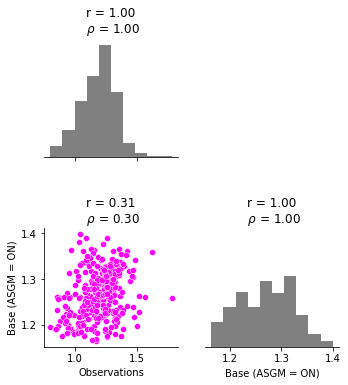
\includegraphics[width = 0.3\linewidth]{templates/figures/GMOS_Sites/sis.png}}\\

% \subfloat[Niew Nickerie]{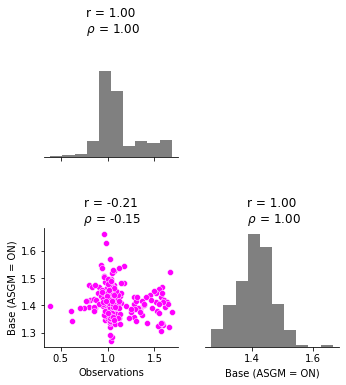
\includegraphics[width = 0.3\linewidth]{templates/figures/GMOS_Sites/NIk.png}} &
% \subfloat[Manaus]{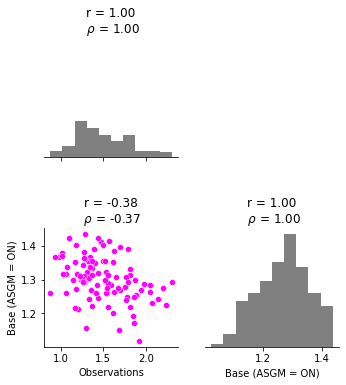
\includegraphics[width = 0.3\linewidth]{templates/figures/GMOS_Sites/man.png}}\\
% \subfloat[Calhau]{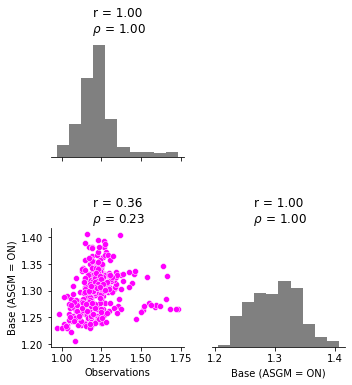
\includegraphics[width = 0.3\linewidth]{templates/figures/GMOS_Sites/cal.png}}
% \end{tabular}
% \centering
% \captionof{figure}{Sensitivity of Observations to Emission Changes in single grid box when the interquartile range (IQR) is used as the metric to compare the observations to model outputs}
% \label{fig:Histplotsiqr}
% \end{figure}
% \FloatBarrier
\subsection{Passive Sampler Observations vs GEOS-Chem}
\begin{figure}[H]
  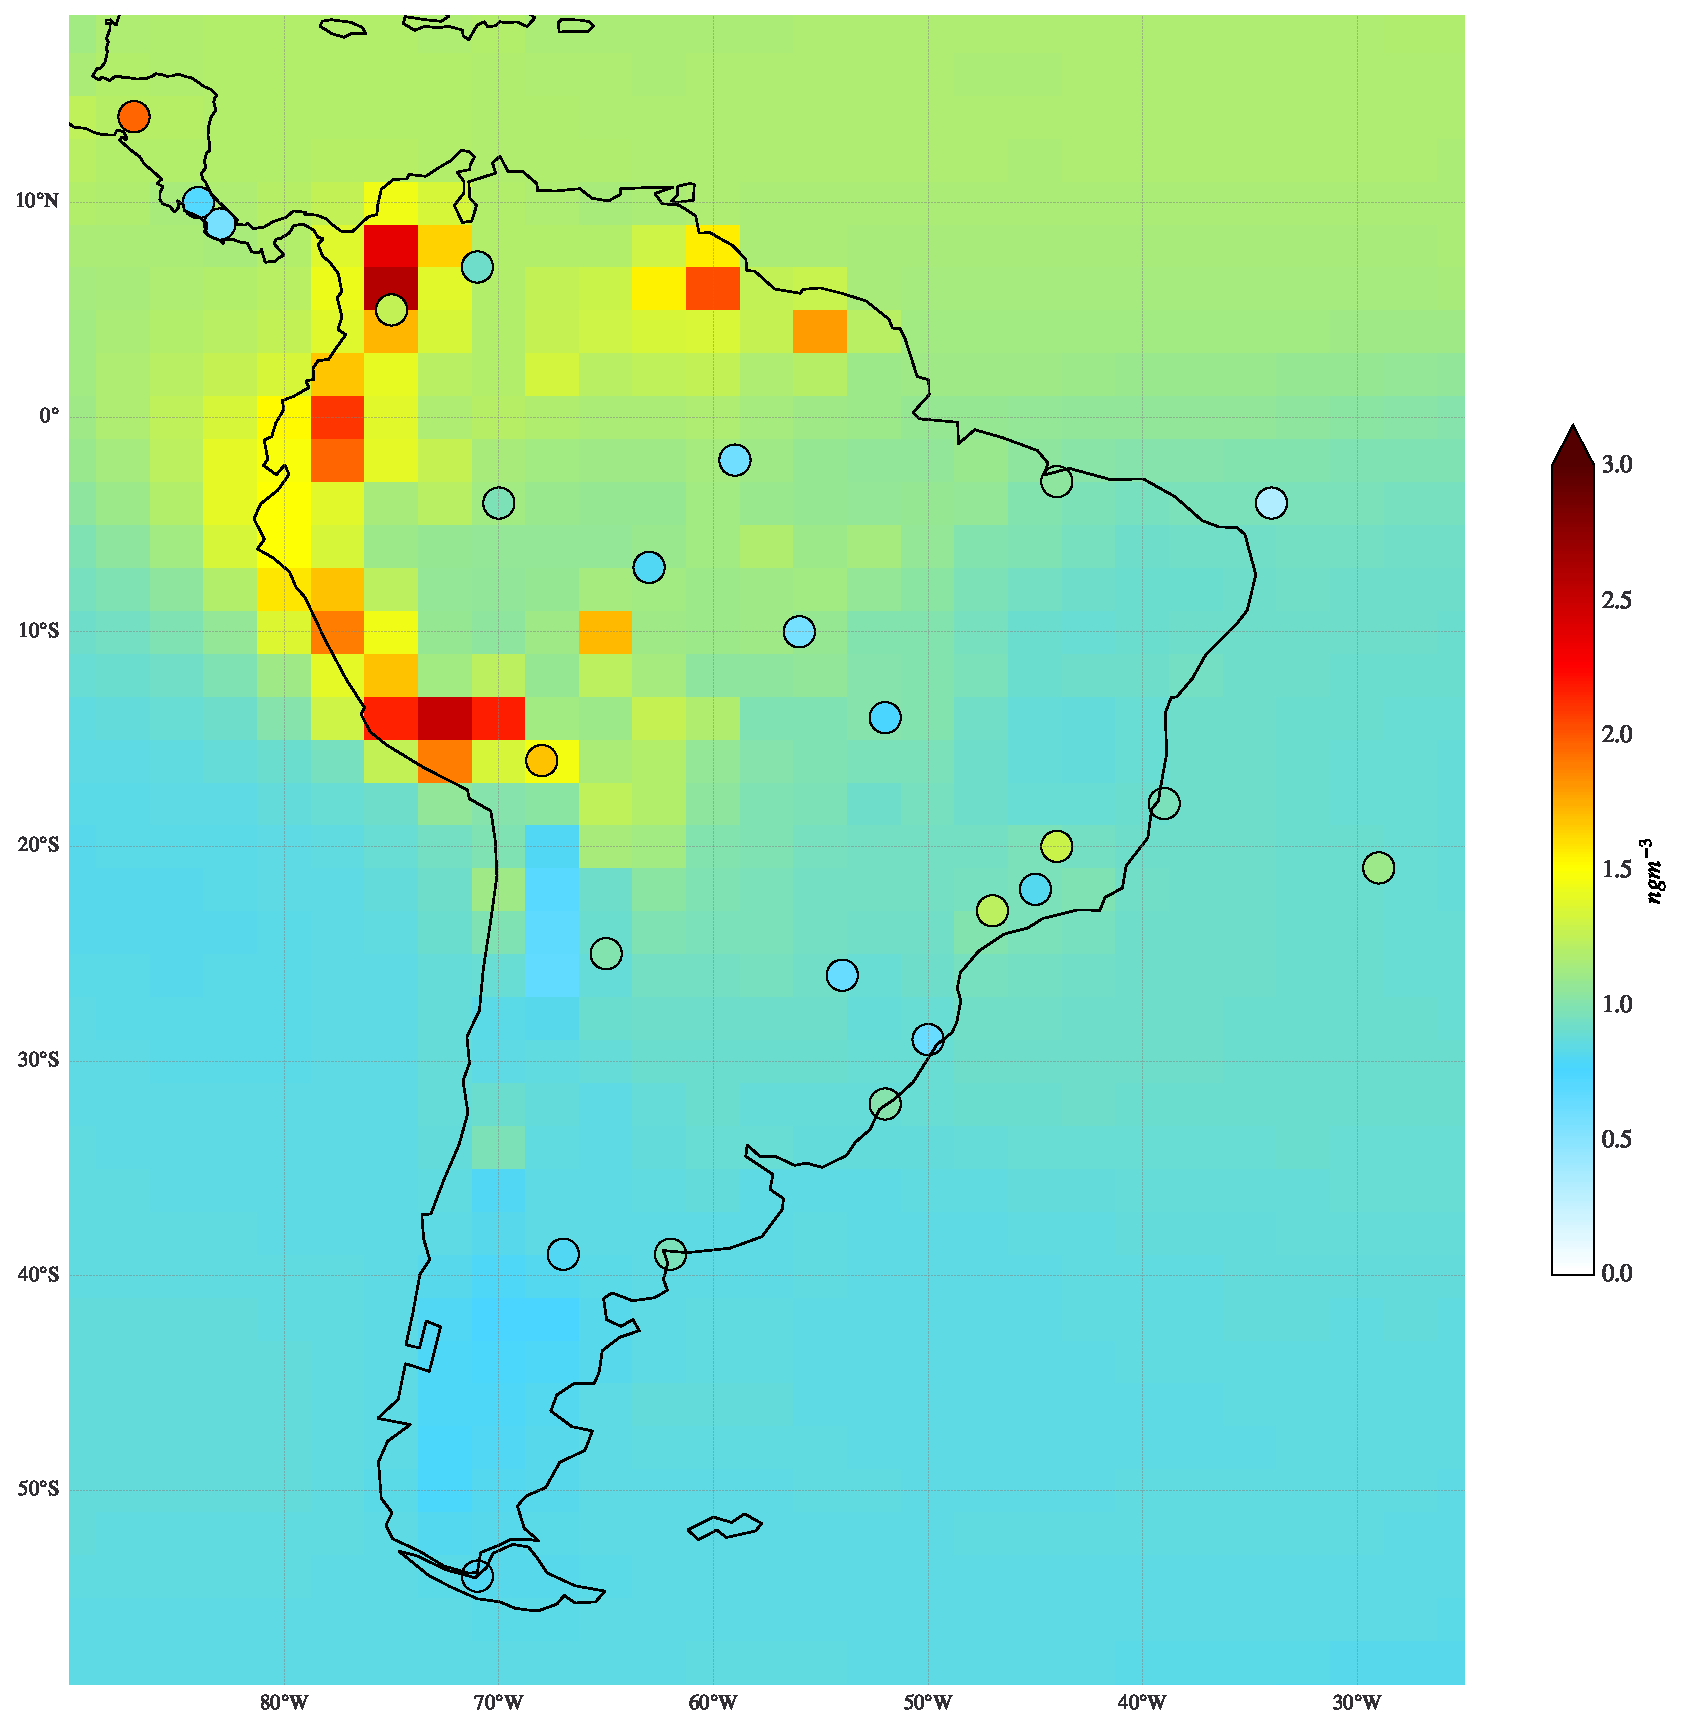
\includegraphics[width=0.7\textwidth]{templates/figures/Passive_Samplers/06-12-22_pas_vs_model_Hg0-per-year_001.pdf}
  \caption{Surface \hg over Latin America averaged over the course of one year, 2015.The figure compares the the annual average \hg produced by the \on (background grid) with the PAS measurements (circles). The PAS measurements are highest in the eastern coastal regions and in the north western region while the model overestimates the concentrations more inland regions.}
  \label{fig:06-12-22_pas_vs_model_Hg0-per-year_001}
  \centering
  
\end{figure}
\FloatBarrier

\begin{flushleft}
 The comparison between the modelled concentration in the atmosphere and the PAS data corroborated the finding that the GEOS-Chem model overestimated the observed concentrations in the atmosphere as seen on Figure \ref{fig:06-12-22_pas_vs_model_Hg0-per-year_by-latitude_001} which show the modeled (blue circles) and observed (red circles) annual average \hg plotted as a function of latitude. The observation error bars are represent the replicate precision of the observations while the model error bars represent the 95\textsuperscript{th} bootstrap confidence interval for the mean anual \hg. Moreover the PAS observations show high variability as you move from South to North while the model has low variability and and increasing trend.  
\end{flushleft}


\begin{figure}[H]
  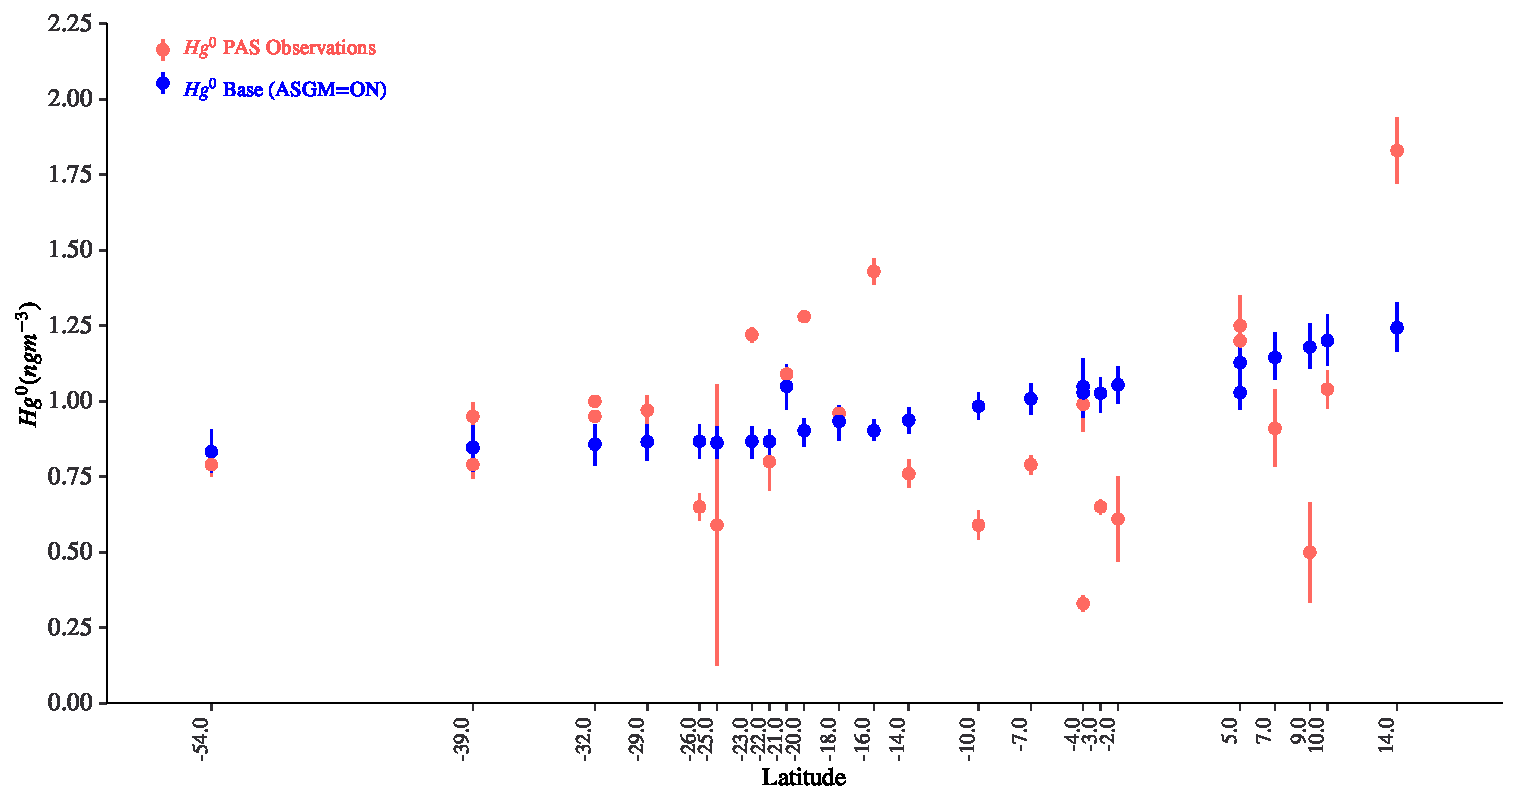
\includegraphics[width=\textwidth]{templates/figures/Passive_Samplers/06-12-22_pas_vs_model_Hg0-per-year_by-latitude_001.pdf}
  \caption{\hg in the atmosphere as a function of Latitude. The \on (blue circles) and observed (red circles) annual average \hg plotted are plotted as a function of latitude to evaluate spatial trends across the continent. The observation error bars are represent the replicate precision of the observations while the model error bars represent the 95\textsuperscript{th} bootstrap confidence interval for the mean annual \hg.}
  \label{fig:06-12-22_pas_vs_model_Hg0-per-year_by-latitude_001}
  \centering
  
\end{figure}
\FloatBarrier



\subsection{Observed Hg Concentration at CHC}
\begin{flushleft}
The time series of the observed concentration at the CHC station between July 2014 and January 2016 is shown on Figure\ref{fig:ObsTseries}. The detailed characteristics of the observations over this measurement period were described in Koening et al.,(2020); hence we will focus the analysis on using the observation TGM data to evaluate the performance of the GEOS-Chem model in predicting the \hg  based on the input \hg emission inventories. As shown by the plot of the \hg 120 day moving as a function of time on Figure\ref{fig:ObsTseries}, we found that the observed TGM concentration in the atmosphere had a visible upward trend, which Koening et al.,(2020) attribute to the El Niño-Southern Oscillation (ENSO). Consequently, Koening et al.,(2020) categorized the measured TGM concentrations in the atmosphere at the CHC site into normal conditions (NC), 2014-07 to 2015-05 and ENSO conditions  2015-06 to 2016-01. The meteorology associated with ENSO was not accounted for in the GEOS-Chem \hg simulations we conducted; therefore the simulated \hg  at CHC was compared to the TGM observations for the one year period between 2014-07-02 to 2015-07-02.
\end{flushleft}

\begin{figure}[H]
  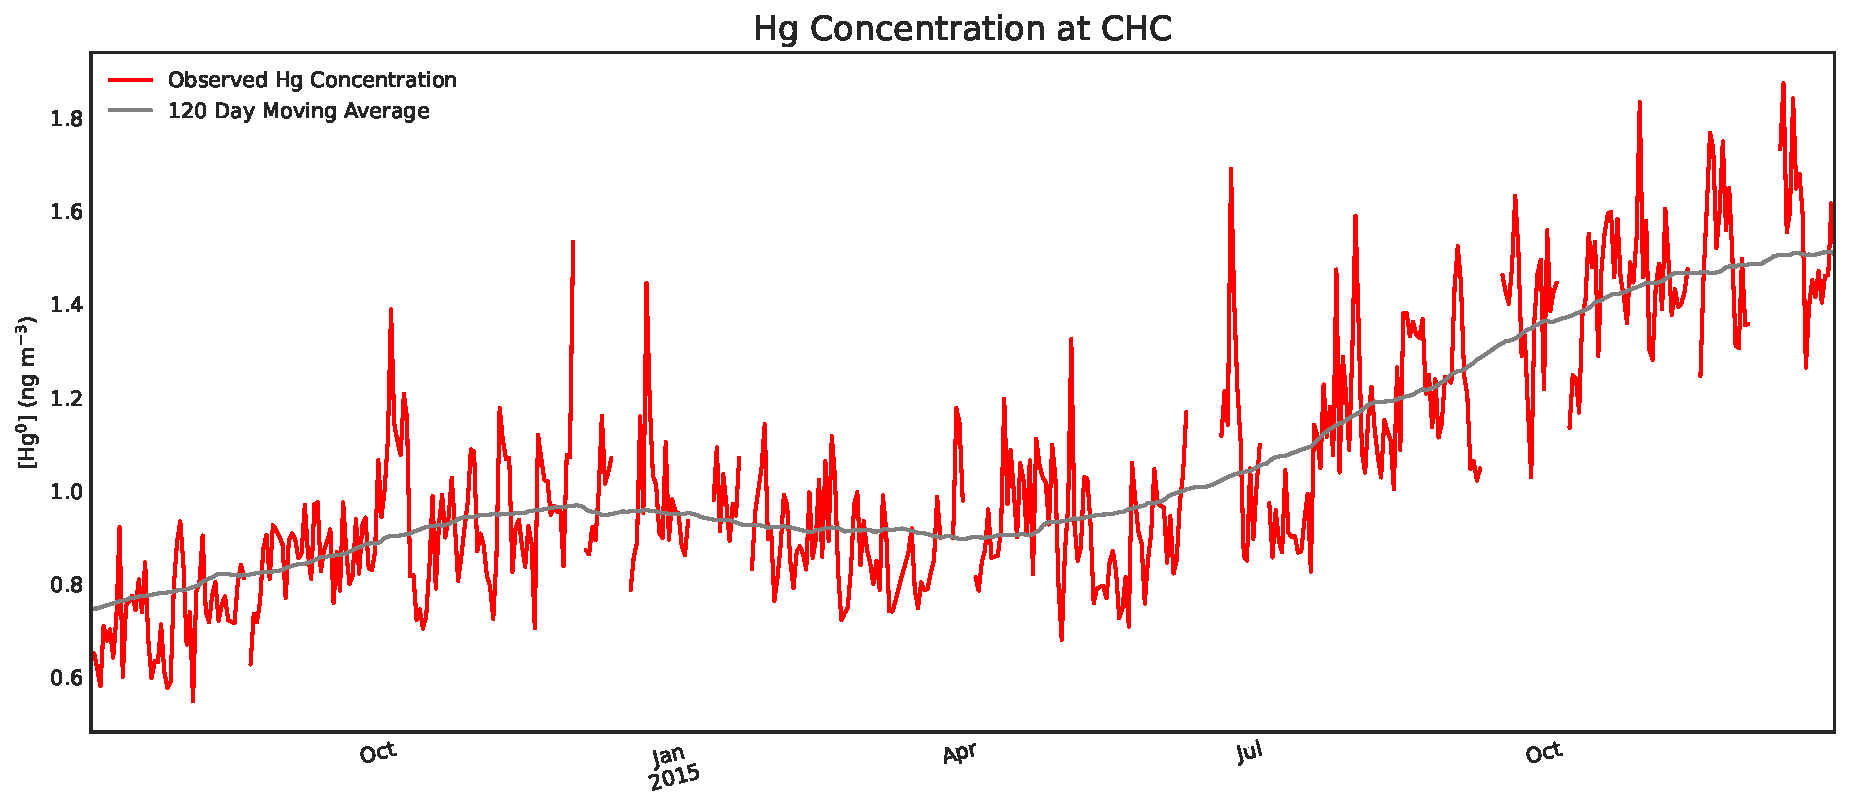
\includegraphics[width=\textwidth]{templates/figures/GMOS_Sites/ObsTimeSeries.pdf}
 
  \caption{The average daily TGM concentration at CHC in ngm\textsuperscript{-3} as a function of time over the measurement period from July 2014 to January 2016. The daily average concentration in indicated by the red line while the grey line shows the 120 day moving average which clearly highlights the upward trend in the daily averages}
  \label{fig:ObsTseries}
  \centering
\end{figure}
\FloatBarrier

\begin{flushleft}
  Figure \ref{fig:ModelvsObsNstats} the detailed comparison between the simulated \hg  and the observed TGM concentration at CHC. The observations (in red) are plotted as a function of time in (a) with the Base (ASGM= OFF) simulation (in green) and (c) with the Base (ASGM= ON) simulation in (blue). The scatter plots in (b) and (d) represent the modeled \hg  as a function of the measured TGM concentration. The scatter plot in plot (b) the variability in the observed TGM concentration is not captured by the Base (ASGM= OFF) simulation while the scatter plot in (d) shows that the Base (ASGM=ON) simulation over estimates the observed values even though it matches the variability in the values. The dispersion around the 1:1 line is substantial in both scatter plots and hence the correlation coefficient is low in both cases. 
\end{flushleft}


\begin{figure}[H]
  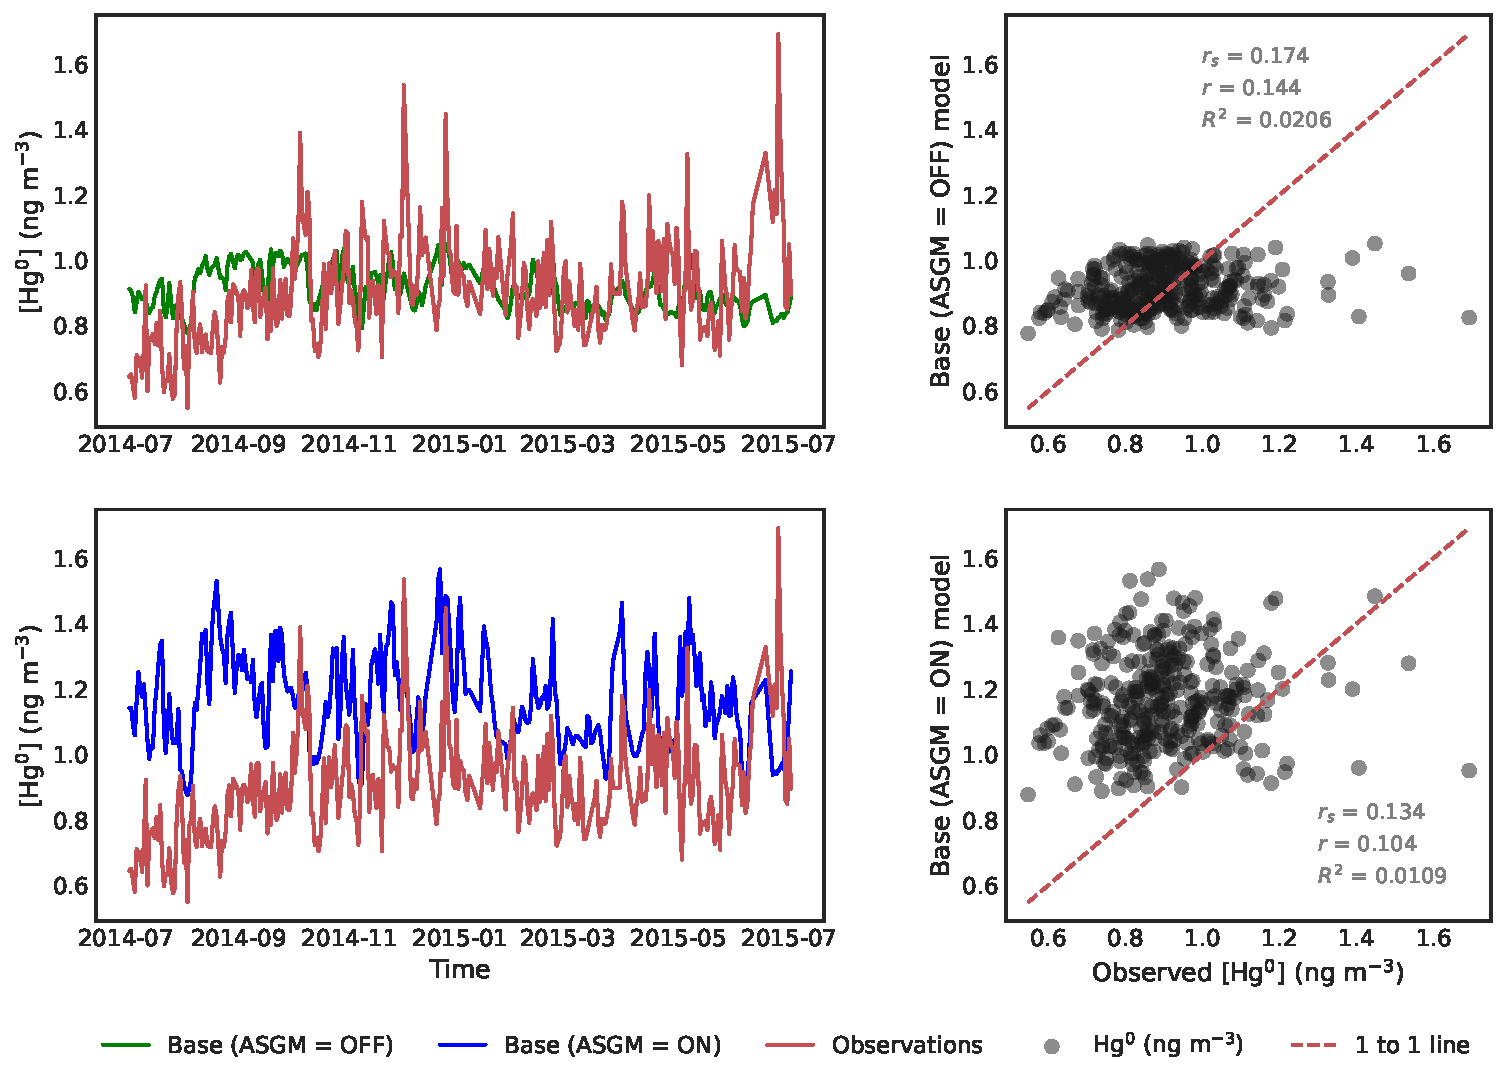
\includegraphics[width=\textwidth]{templates/figures/ModelvsObs/TimeSeriesNsactter_obsVmodel_v1.pdf}
  \centering
  \caption{Observed vs modelled (3 different simulations) Hg concentration at CHC and scatter plots of how the model compares with the observations  }
  \label{fig:ModelvsObsNstats}
\end{figure}
\FloatBarrier
\begin{flushleft}
We also found that the mean \hg concentration produced by the Base (ASGM= OFF) simulation was within 1\% of the observed TGM concentration as seen on Table \ref{tab:ModelvsObsStats} where$\mu$ is the annual average Hg concentration, $\sigma$ is the standard deviation, $iqr$ is the interquartile range, $r_s$ is the Spearman correlation, $r$ is the Pearson correlation and $R^2$ is the coefficient of determination. On the contrary, the average \hg produced by the \on shown by the blue line plot on Figure \ref{fig:ModelvsObsNstats} overestimated the mean by 29\%.
 
\end{flushleft}
\setlength{\tabcolsep}{2.5pt}
\begin{table}[H]
  \begin{center}
    \caption{Characteristics of observed and modelled Hg concentration in CHC where$\mu$ is the annual average Hg concentration, $\sigma$ is the standard deviation, $iqr$ is the interquartile range, $r_s$ is the Spearman correlation, $r$ is the Pearson correlation and $R^2$ is the coeeficient of determination}
    \label{tab:ModelvsObsStats}
    \begin{tabular}{lcccccc}
       %<-- added & and content for each column
      
                          & $\mu$                 & $\sigma$            & $iqr$               & & & \\
                          &  (ng m$^{-3}$)/year)  & (ng m$^{-3}$)/year) & (ng m$^{-3}$)/year) & & & \\
     \cmidrule{2-4}
     Observations         & 0.90             & 0.16            & 0.18        &  & & \\
     \textbf{Simulations} &                  &                  &               &\textbf{$r_s$} &\textbf{$r$} &\textbf{$R^2$}\\ %
      \hline
      Base (ASGM=OFF)     & 0.91             & 0.06            & 0.11         & 0.17         & 0.144      & 0.0196\\ 
      Base (ASGM=ON)      & 1.16            & 0.14            & 0.20        & 0.124         & 0.101       & 0.0102\\ % <--
    \end{tabular}
  \end{center}
\end{table}
\FloatBarrier

\begin{flushleft}
Even though GEOS-Chem reproduced the mean Hg concentrations at CHC in the \off, the Spearman ($r_s$) and Pearson ($r$) correlations between the modelled and observed concentrations were very low at 1.63e-1 and 1.40e-1 respectively. Moreover, the coefficient of determination, $R^2$ between the observed and modelled concentrations in \on case was almost zero at 0.021. Also, the \on did not reproduce the variability in the observed concentrations as evident in Figure \ref{fig:ModelvsObsNstats} and in Table \ref{tab:ModelvsObsStats} where we gleaned that the observations had more than twice the modelled variance in the \on case. Brasseur et al.,(p.471 2017) assert that in cases where a model captures the observed means but not the observed variability, the mean may be wrongly interpreted \cite{brasseur_modeling_2017}.  In addition, we found that turning on ASGM emissions in GEOS-Chem led to \hg s in the atmosphere that had a variance that is comparable with the observed variance. However, we also discovered that turning on ASGM emissions in the model did not lead to improvements in the correlation between the modeled and observed \hg in the atmosphere. 
The relationship between the mean and variance in the observed and modeled Hg concentration in the atmosphere at CHC was further explored as shown on Figure \ref{fig:Histplots} which shows the extent to which the GEOS-Chem model reproduces the mean and IQR of the observations. Even though the \on  better recreated the IQR of the Hg concentration in the atmosphere, the mean \hg in this simulation was almost two standard deviations away from the mean of the observations. The above comparison indicates that the mean was not a good metric to investigate the relationship between the Hg concentration in the atmosphere and ASGM emissions as modelled by GEOS-Chem. 
\end{flushleft}



\begin{figure}[H]

\begin{tabular}[H]{cc}

\subfloat[]{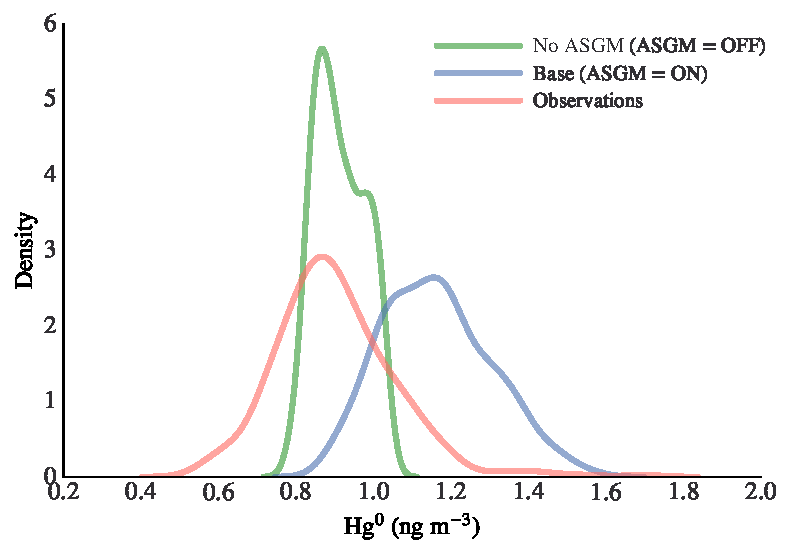
\includegraphics[width = 0.5\linewidth]{templates/figures/ModelvsObs/06-12-22_models_vs_observations_density-plot.pdf}} &
\subfloat[]{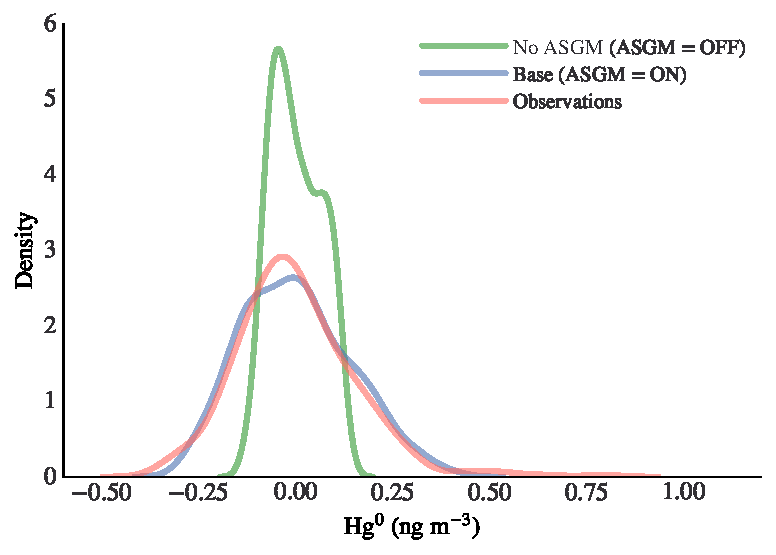
\includegraphics[width = 0.5\linewidth]{templates/figures/ModelvsObs/06-12-22_models_vs_observations_density-plot_std.pdf}}
\end{tabular}
\centering
\captionof{figure}{Plots Showing Data and Modeling  Results from GMOS Monitoring Network Sites in South America}
\label{fig:Histplots}
\end{figure}
\FloatBarrier

\begin{flushleft}
Instead, the IQR and 95$^{th}$ percentile range were found to be metrics that were informative about the effect of ASGM on the simulated Hg concentration site at distant high altitude measuring station site. The failure of GEOS-Chem to reproduce the observed mean Hg concentration at a high altitude measuring site may be attributed to poor parameterizations in the model such as the influence of dry deposition. The flaws in the GEOS-Chem Hg dry deposition scheme in version 12.8.1 of GEOS-Chem used in this analysis were discussed in detail and improved in Feinberg et.al (2022). Furthermore, we hypothesized that poor spatial distribution of emissions in the 2015 Hg ASGM emissions inventory which are an input to the GEOS-Chem may have also contributed to the model observation mismatches. 

\end{flushleft}






\section{Conclusion}

